

\hypertarget{introduction}{%
	\section{Introduction}\label{introduction}}

\begin{figure}[h!]
	\centering
	\includegraphics[width=0.7\textwidth]{chap1ruysch.png}
	\caption{\label{fig_1_1} \textbf{The Anatomy Lesson of Dr.~Frederik Ruysch}, 1670 by
		Adriaen Backer. \cite{ruyshc}}
\end{figure}

The term ``epithelia'' was first introduced by Dutch botanist Frederick Ruysch in the early 18th century (see Fig. \ref{fig_1_1}). He used it to describe the tissue he observed while dissecting the lips of a cadaver, and the word is derived from Greek roots ``epi,'' meaning top, and ``thele,'' meaning nipple.\footnote{Ruysch is referred to as a ``Artist of death'' because of his famous anatomical collection. He was the first to use arterial embalming, which allowed for visualizing and dissecting smallest arteries. He also was part of the macabre practice of public dissections \cite{halley2019}.}
A few decades later, Swiss scientist Albrecht von Haller began using the term ``epithelium/epithelia'' to describe the fibers of the body, following the old Renaissance theory that the body was made of fibers, which were believed to be a fundamental building block of living things.\footnote{Finding a fundamental unit of living entities comes from the philosophy of Gottfried W. Leibniz. It was based on the idea of ``monad''. Thanks to progress in microscopy and philosophy, naturalists were able to put together ideas for cells, fibers, and even cytoskeleton! \cite{zampieri2014}}
It was thought that these fibers and tissues arranged in different arrays gave rise to biological structures \cite{maccord2012, zampieri2014}. This theory was not far off, as epithelial tissues make up more than 60\% of the cells in a vertebrate's body and are found ubiquitously, covering the organs both inside and out \cite{alberts2015}.

Epithelial cells are polarized, i.e., their apical side (typically facing the lumen of the organ), which differs in shape and composition from the basolateral side. Its polar organization is reflected in the vectorial functions like creating and maintaining concentration gradients between separated compartments \cite{marchiando2010}. Typical examples of these are transporting epithelia such as those of the renal tubule, absorptive epithelia of the intestine, and secretory epithelial cells like hepatocytes \cite{alberts2015}. In addition, polarized epithelia guide the developmental process by determining the fate of cells leading to symmetry-breaking events in the embryo \cite{kim2018}.

\hypertarget{key-components}{%
	\section{Key components}\label{key-components}}

The function of epithelia primarily depends on the tissue's structure and the surrounding microenvironment. It can be divided into three aspects: cell structure, microenvironment, and cell-matrix interactions.

\hypertarget{cell-structure}{%
	\subsection{Cell structure}\label{cell-structure}}

The cell cytoskeleton plays a crucial role in maintaining cell shape and supporting vital functions such as cell division and migration \cite{alberts2015}. The Eukaryotic cell cytoskeleton is composed primarily of filamentous proteins, including three main types of filaments that differ in size and protein composition: microtubules, actin filaments, and intermediate filaments (see Fig. \ref{fig_1_3b}). Microtubules, with a diameter of approximately 25 nm, are the largest and made of the protein tubulin. Actin filaments, with a diameter of only 6 nm, are the smallest. Intermediate filaments, with a diameter of around 10 nm, are composed of several different subunit proteins and have a diameter intermediate between the other two types \cite{mofrad2009}. All three filament types dynamically respond to signals from the microenvironment and cell networks.

Mechanically, microtubules have higher extensional stiffness than  actin filaments but break at lower extensions. Intermediate filaments have intermediate extensional stiffness and can sustain larger extensions while showing a nonlinear stiffening response \cite{wen2011}. Differences in strength and stability arise from the properties of individual subunits. The persistence length can range from 1\unit{\um} for intermediate filaments to 1\unit{\mm} for microtubules \cite{fletcher2010}. Actin filaments, most relevant to this thesis, have a persistence length of a few microns.

The assembly and disassembly of these filaments are dictated by the dynamics of their macromolecular components and accompanying proteins. The combination of actin filaments and myosin motors forms the actomyosin cortex, which is essential in producing intra- and intercellular forces. In an epithelial tissue, the actomyosin cortex and intercellular junctions make cell-to-cell contacts stronger and provide tissue integrity \cite{braga2016} (see Fig. \ref{fig_1_3}). A good example of these tissue-level structures can be observed in wound healing assays, where cells surrounding the wound create a ring of actin to close it \cite{brugues2014}. In Chapter 3, we will delve into the actomyosin network in more detail.

\begin{figure}[h!]
	\centering
	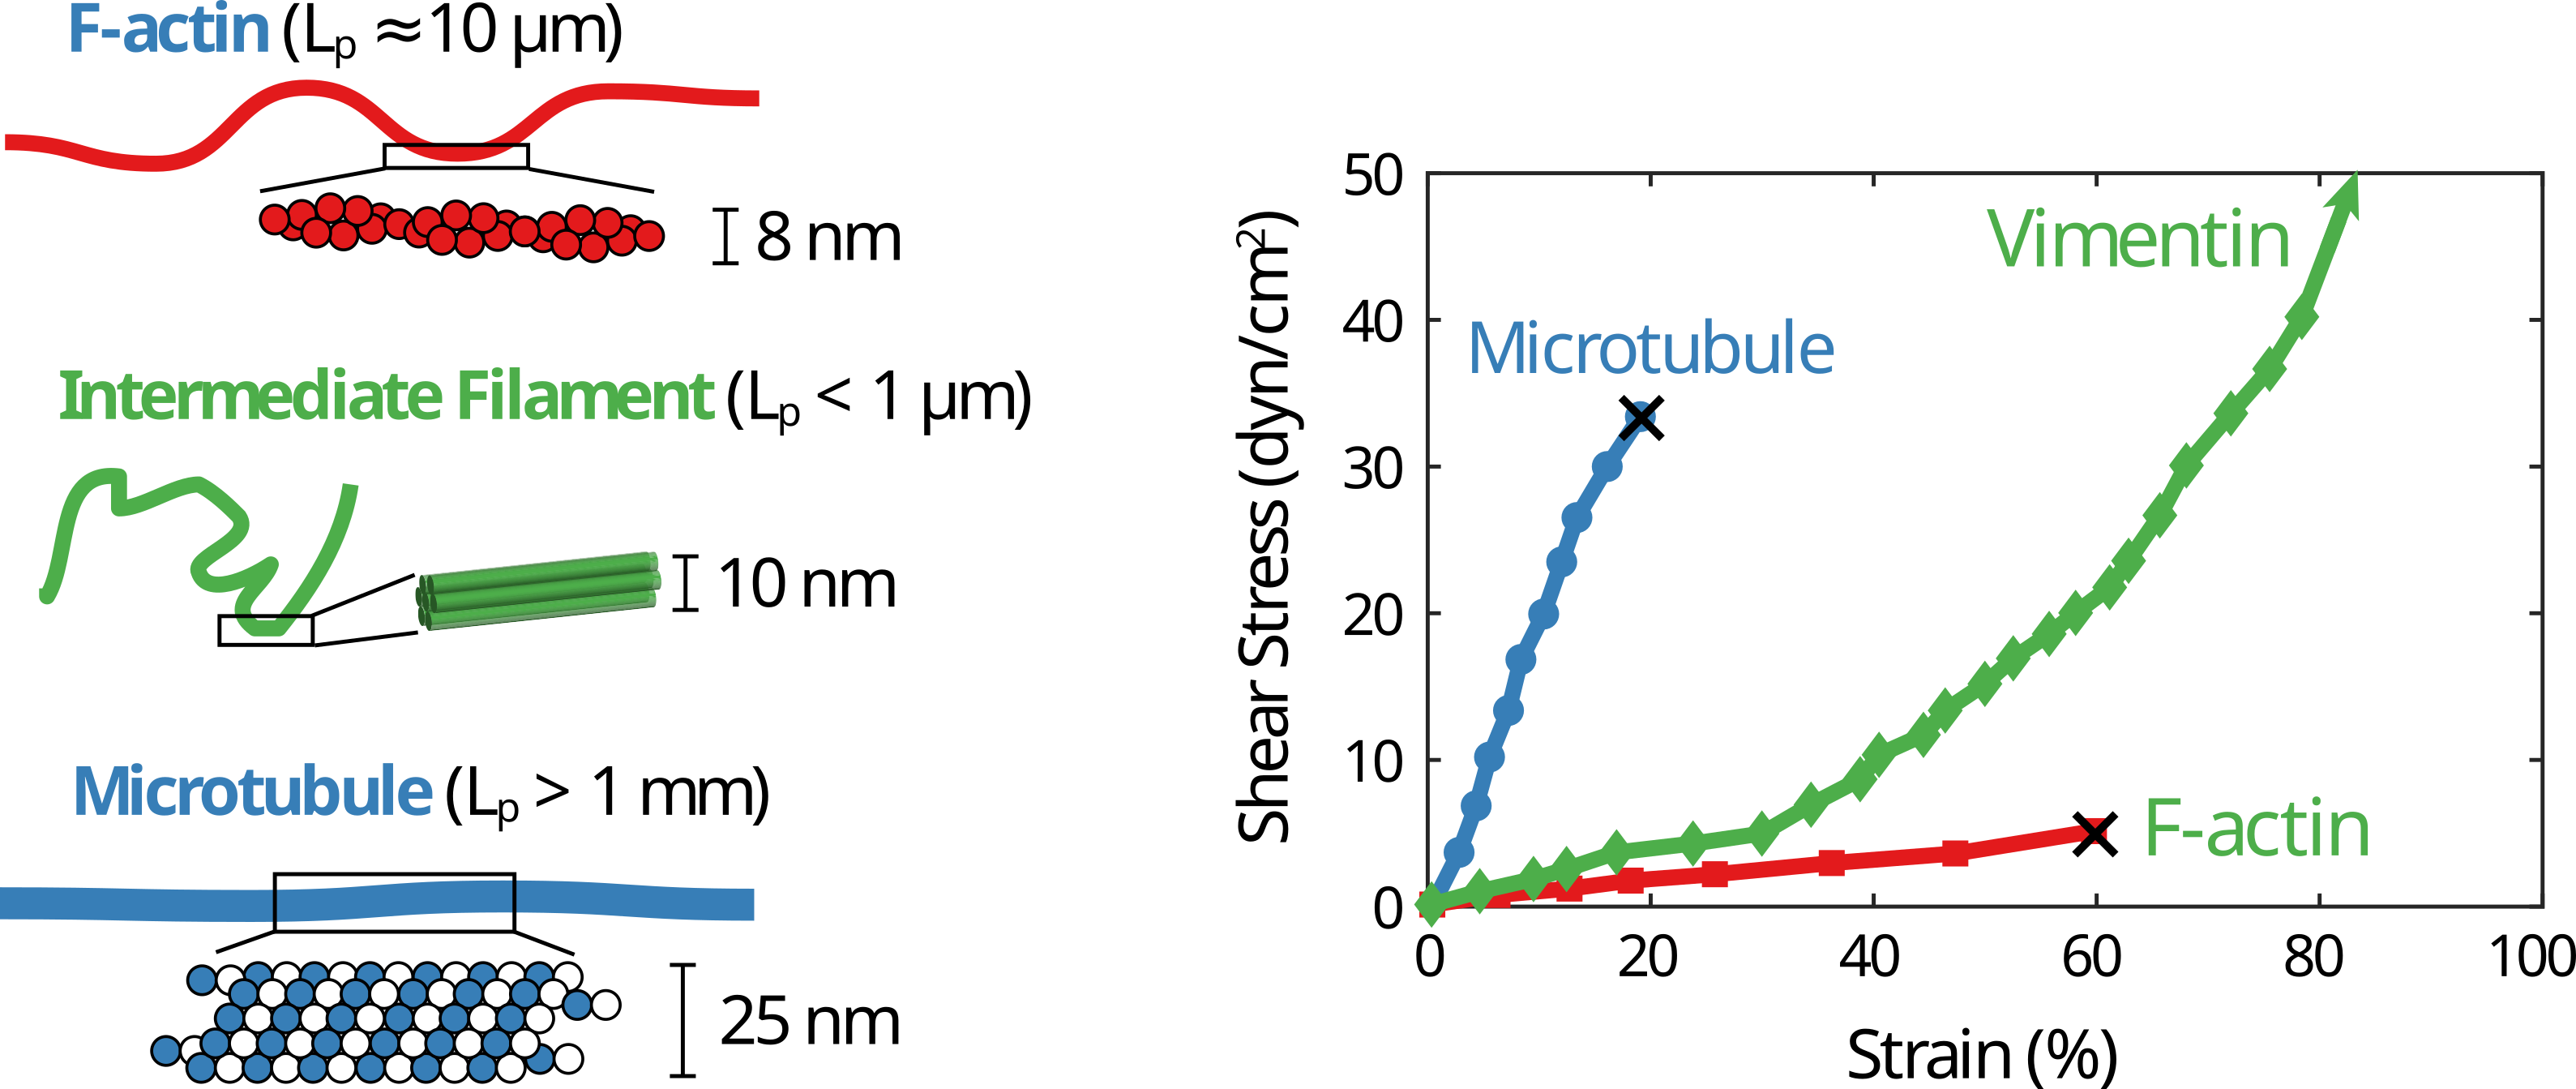
\includegraphics[width=0.8\textwidth]{chap1_filaments.png}
	\caption{\label{fig_1_3b} \textbf{Mechanics of cytoskeletal filaments}: Schematic and sizes of actin filaments, intermediate filaments and microtubules; along with the strain response to shear stress. \textit{Adapted from \cite{leggett2021}}}
\end{figure}

Multiple membrane molecules can facilitate cell adhesion, including cadherins. Cadherins are a crucial component for epithelial cell cohesion and the formation of adherens junctions, which transmit forces between cells. This key factor is involved in the mechanical regulation of cell division and tissue rearrangement during development and homeostasis \cite{godard2019, mertz2013}. Desmosomes, another type of intercellular junction, are coupled with intermediate filaments and provide mechanical resilience to cell layers \cite{hatzfeld2017, latorre2018}. Tight junctions serve as a barrier and regulate the active transport of ions across epithelial layers, playing an important role in controlling fluid pressure in tissues \cite{marchiando2010, chan2020}.

\begin{figure}[H]
	\centering
	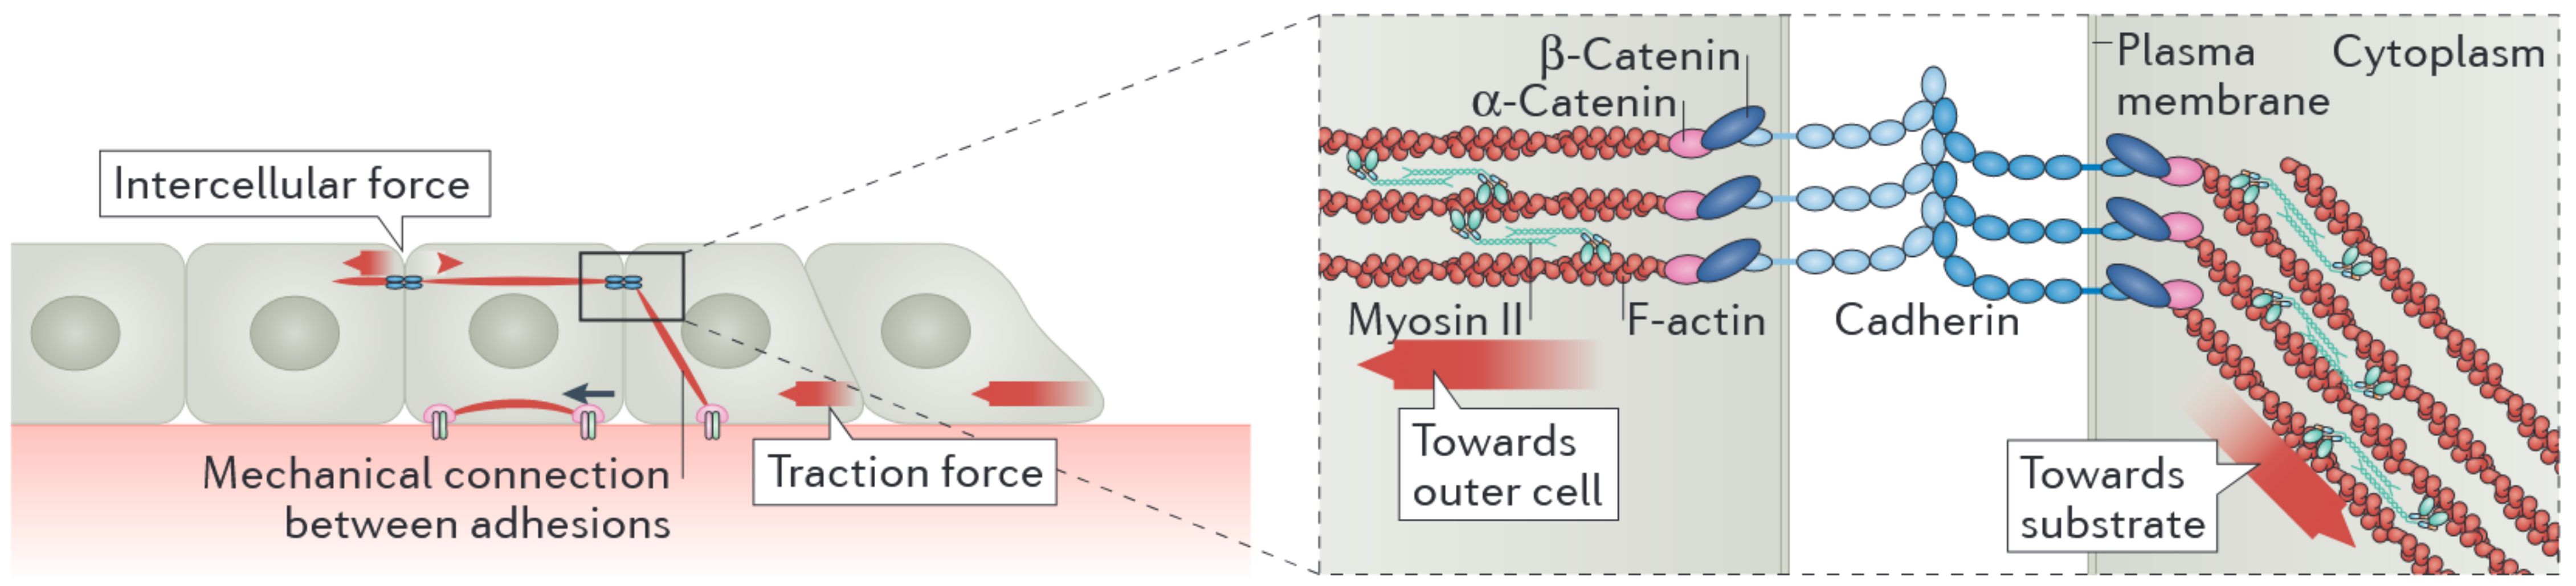
\includegraphics[width=\textwidth]{chap1_cellforces.png}
	\caption{\label{fig_1_3} \textbf{Intercellular forces through actomyosin cables and cadherins}: Schematic showing mechanical connections between adhesions and tissue force transmission with actomyosin cytoskeleton and adhesion proteins. \textit{Adapted from \cite{ladoux2017}}}
\end{figure}

\hypertarget{microenvironment}{%
	\subsection{Microenvironment}\label{microenvironment}}

The extracellular matrix (ECM) is the substrate or cell environment to which cells adhere. It is also referred to as the matrix, mesenchyme, or cellular microenvironment. The ECM serves many functions. It endows tissues with strength, thereby maintaining their shape. Additionally, it serves as a biologically active scaffolding that allows cells to migrate or adhere. The ECM also plays a role in regulating the phenotype of cells. It provides an aqueous environment that facilitates the diffusion of nutrients, ions, hormones, and metabolites between the cell and the capillary network \cite{alberts2015}.

Moreover, the ECM is subjected to mechanical forces such as blood flow in endothelia, air flow in respiratory epithelia, or hydrostatic pressure in the mammary gland and bladder \cite{waters2012, walma2020}. It has been shown that the ECM regulates cell shape, orientation, movement, and overall function in response to biophysical forces \cite{alberts2015}.

The ECM is a fibrous network of proteins, consisting of collagen, elastin, and proteoglycans as its primary structural components. Collagen is one of the most abundant proteins in the body, while elastin is the most elastic and chemically stable protein. Proteoglycans can sequester significant water as well as growth factors and proteases. The water content of the ECM allows it to deform as a poroelastic material, absorbing water upon stretching and releasing it under compression, causing a hydraulic fracture effect \cite{casares2015}. The collagen network can also remodel under the influence of cells and mechanical forces \cite{humphrey2014}.

Most ECM components undergo continuous turnover, some quickly and some slowly. For example, the half-life of collagen in the periodontal ligament is a few days, whereas that in the vasculature may be several months \cite{humphrey2014}. In response to altered physical stimuli, disease, or injury, the rates of collagen synthesis and degradation can increase many times, allowing for a rapid response.

\hypertarget{cell-matrix-interaction}{%
	\subsection{Cell-Matrix interaction}\label{cell-matrix-interaction}}

The cells and the extracellular matrix (ECM) are in a dynamic relationship, constantly exchanging information and influencing each other. The cells sense the biophysical cues in the ECM through sensors such as integrins and focal adhesion complexes, which are responsible for cell-substrate adhesion \cite{kechagia2019} (see Fig. \ref{fig_1_4}). These adhesions allow cells to respond to various stimuli such as matrix stiffness, ligand density, and chemotactic gradients \cite{fortunato2022}. It has also been shown that cells can respond to the viscoelasticity of the matrix \cite{elosegui-artola2022}.

\begin{figure}[h]
	\centering
	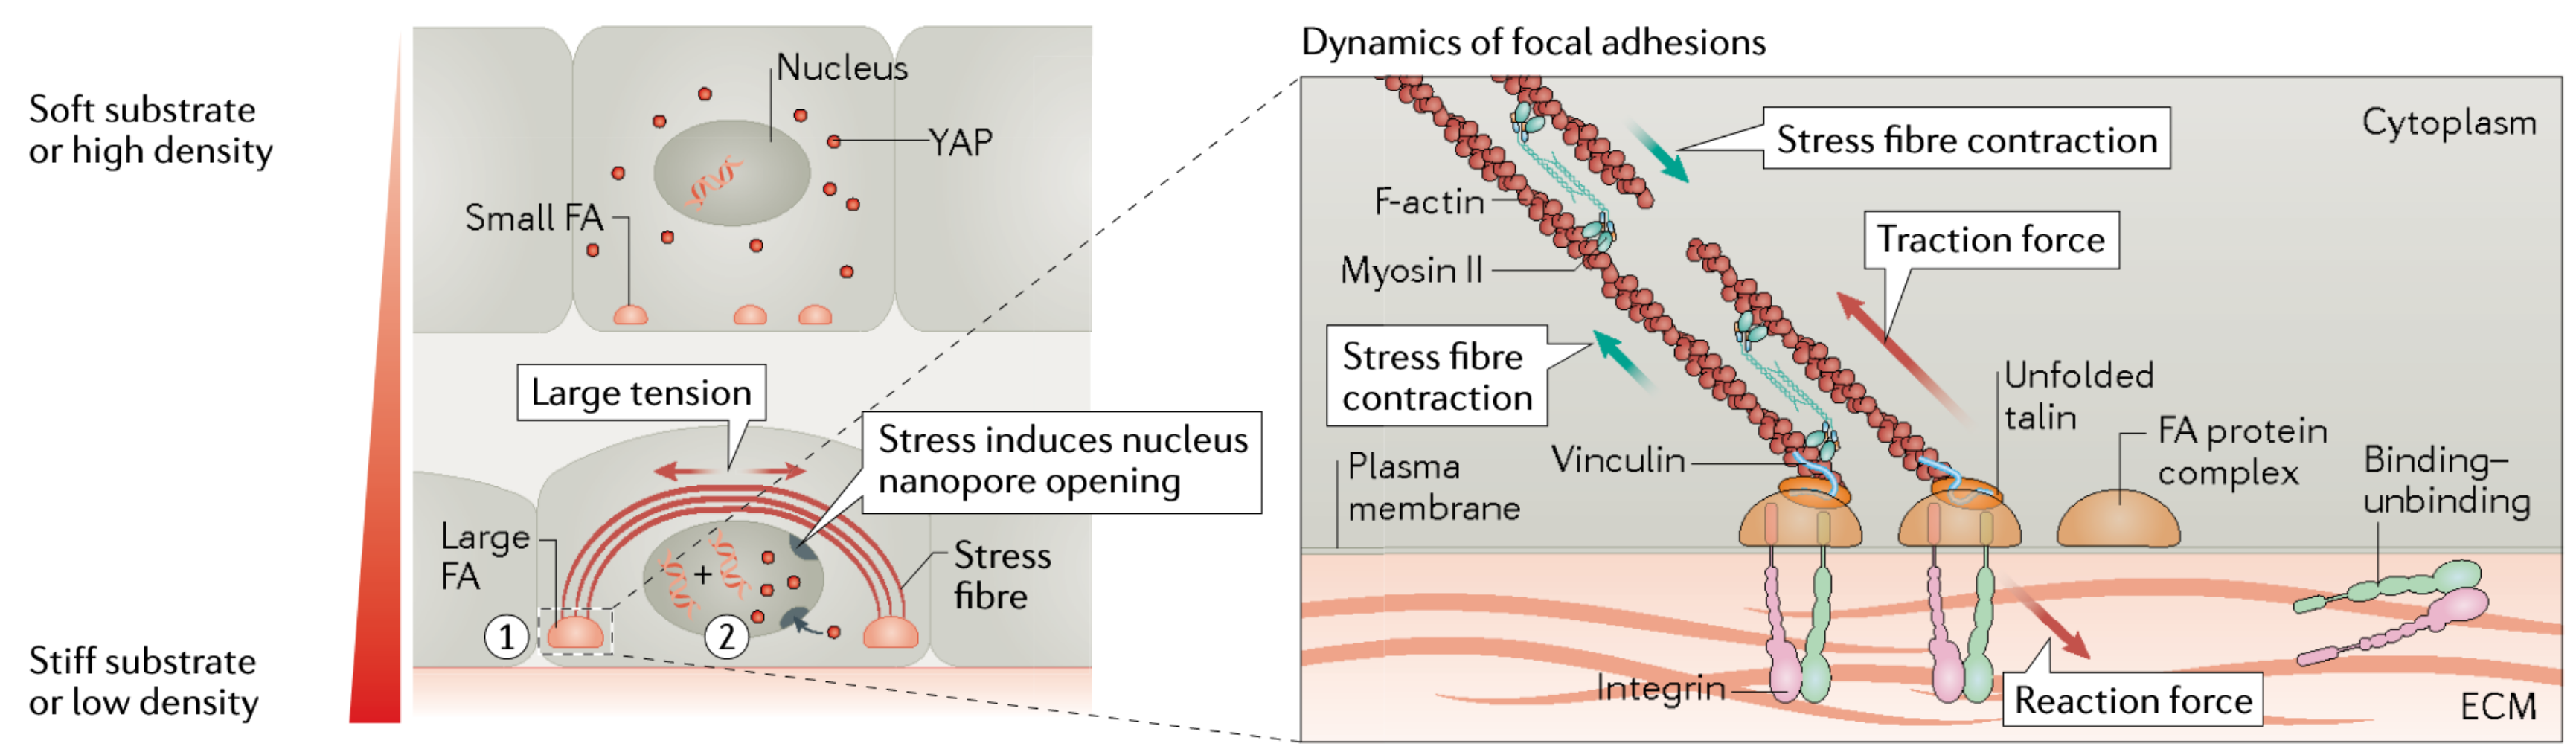
\includegraphics[width=\textwidth]{chap1_cell-matrix.png}
	\caption{\label{fig_1_4} \textbf{Cell-matrix interaction with respect to matrix stiffness and cell density}: In higher tension condition, the nucleus is deformed triggering mechanotransduction and causing alterations in cytoskeleton and tractions. \textit{Adapted from \cite{xi2018}}}
\end{figure}

In addition to sensing the ECM, cells also contribute to its composition by secreting ECM components or remodeling the substrate \cite{malandrino2018}. This interplay between the cells and ECM can impact the tissue behavior fundamentally, as the connections between focal adhesions and the nucleus can affect the expression of transcriptional factors \cite{venturini2020, lomakin2020}. The precise control of cell-cell and cell-substrate interactions enables cells to transform into intricate shapes, such as curved forms in cell sheets \cite{schamberger2022}.

%\hypertarget{role-in-disease-and-development}{%
%	\section{Role in disease and
%		development}\label{role-in-disease-and-development}}
%
%Maintaining epithelial integrity and homeostasis is crucial for survival, and mechanisms have evolved to ensure these processes are sustained during growth and in response to damage. Epithelial cells have one of the fastest turnover rates in the body, with the entire gut cell lining turning over in 5--7 days \cite{barker2014}. This constant cell division and death pose a risk for tumor formation; it is know that 90\% of cancers emerging in simple epithelia \cite{torras2018, eisenhoffer2013}. Additionally, the high rate of cell turnover can disrupt the barrier function, as gaps should not emerge around dividing or dying cells.
%
%If the fluid compartmentalization goes awry, it can have profound implications for epithelial and stromal homeostasis, fluid and electrolyte balance, and the development of inflammatory states. Several bacterial toxins are known to target junctions, causing changes in the tight junction protein ZO1, which compromises the barrier function and leads to pathologies such as diarrhea and colitis \cite{fasano1991}. In cancer, the compromised ZO1 barrier is essential to allow metastatic cells to break into and out of blood vessels. The leaky barrier also enables a growing epithelial tumor to access luminal fluids as an additional source of nutrients \cite{mullin2005}.
%
%Furthermore, epithelia participate in physiological events such as epithelial--mesenchymal transition (EMT), which is a developmental process where epithelial cells gradually transform into mesenchymal-like cells by losing their epithelial functionality. EMT plays a vital role in normal biological functions such as repair and differentiation, as well as abnormal pathological activity such as organ fibrosis and promoting carcinoma progression \cite{alberts2015}. EMT endows cells with stem cell properties, enabling cell migration to distant organs and subsequent differentiation into multiple cell types during development and the initiation of metastasis \cite{thiery2009}. 
%
%Epithelia undergo drastic shape changes with deformation and reorganization from the embryonic to the adult stage. It's not surprising that any malfunction in this process can lead to damage and disorder, resulting in congenital malformations, which are a major cause of infant mortality worldwide \cite{clarke2021}. Additionally, epithelial dysfunction is a precursor to diseases such as chronic obstructive pulmonary disease, asthma, cystic fibrosis, and pulmonary fibrosis \cite{carlier2021}.

\hypertarget{forms-of-epithelia}{%
	\section{Forms of epithelia}\label{forms-of-epithelia}}

The structure and arrangement of epithelial cells are crucial for maintaining the integrity and homeostasis of tissues and organs (see Fig. \ref{fig_1_5}). Simple epithelia are single-cell layers where all cells are in contact with the underlying basal lamina and have a free surface on the apical side. The shape of the cells can vary, ranging from flat to cuboidal to columnar. Stratified epithelia, on the other hand, have two or more layers of cells. Additionally, there are pseudostratified epithelia, which appear to be stratified, but are monolayers where the cell nuclei are positioned in a manner that gives the appearance of a stratified epithelium.

\begin{figure}[h]
	\centering
	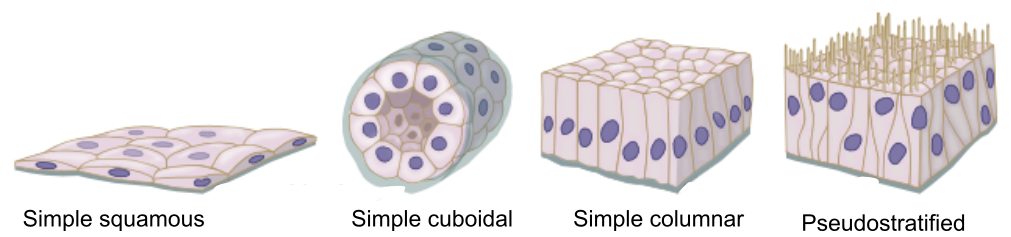
\includegraphics[width=\textwidth]{chap1_forms.png}
	\caption{\label{fig_1_5} \textbf{Forms of epithelial tissues}: Simple squamous, cuboidal, columnar epithelia and pseudostratified epithelia. \textit{Adapted from \cite{zotero-9680}}}
\end{figure}

The classification of epithelia was first established in the XIXth century based on their structure and physiological characteristics. Germ layer theory, developed by embryologists, further expanded the epithelial nomenclature \cite{maccord2012}. During early embryogenesis, three layers emerge: endoderm, mesoderm, and ectoderm. The ectoderm forms the epithelia lining the skin, mouth, and nervous system, while the endoderm gives rise to the digestive tract, respiratory system, and liver. The mesoderm, in turn, develops the endothelia covering much of the circulatory and lymphatic systems.

It is important to note that not all tissues classified as epithelia, mentioned in this thesis, are purely composed of epithelial cells. They may be a mixture of different cell types that have epithelial-like characteristics. The focus of this thesis is on packed cell monolayers, which can form and self-organize into various 3D shapes, ranging from simple spheres to complex branched tubules. The thesis will explore the role of mechanics in epithelial morphogenesis.